\documentclass[../../main.tex]{subfiles}
\begin{document}
\section{Free-free Timoshenko beam}\label{sec:Timo:Free}
Consider a free-free Timoshenko beam model (Problem T-4 in section \ref{ssec:1D_Model:ModelProblems}).The eigenvalue problem of Problem T-4 is denoted by Problem T-4E. Similar to the previous section, this section serves as an example of the application of the theory from [VV02].\\

Consider the general solutions of the eigenvalue problem for the three cases $\lambda < \alpha$, $\lambda = \alpha$ and $\lambda > \alpha$. Imposing the boundary conditions $x = 0$ results in the following:

\begin{align}
	C  =&  \frac{\omega}{\mu}A &\textrm{ and } \ D = \frac{ \mu^2+\lambda}{\omega^2-\lambda}B \ \ \ \textrm{ if } \lambda < \alpha \label{A1}\\
	C = & \frac{\omega}{\lambda}A \ &\textrm{ and } \ D = \frac{\alpha}{\omega^2-\lambda}B  \ \textrm{ if } \lambda = \alpha \label{A2}\\
	C= &-\frac{\omega}{\theta}A \ &\textrm{ and } \ D = -\frac{\theta^2-\lambda}{\omega^2 - \lambda}B  \ \textrm{ if } \lambda > \alpha \label{A3}
\end{align}
The boundary conditions at $x = 1$ gives the following homogeneous system of equations for each of the three cases.
\begin{align}
	\begin{bmatrix}
		M_{11}(\lambda) & M_{12}(\lambda)\\
		M_{21}(\lambda) & M_{22}(\lambda)
	\end{bmatrix}
	\begin{bmatrix}
		A\\
		B
	\end{bmatrix}
	= 
	\begin{bmatrix}
		0\\
		0
	\end{bmatrix}
	\label{eq:Timo:Free:SystemOfEquations}
\end{align}

The entries of the coefficient matrix for each separate case is presented below.

{If $\lambda < \alpha$}
\begin{align*}
	&M_{11}(\lambda) = \sinh(\mu)(\lambda+\mu^2) + \frac{\omega(\lambda - \omega^2)}{\mu}\sin(\omega)&\\
	&M_{12}(\lambda) = (\lambda+\mu^2)(\cosh(\mu)-\cos(\omega))& \\
	&M_{21}(\lambda) = \frac{\lambda}{\mu}(\cos(\omega) - \cosh(\mu))&\\
	&M_{22}(\lambda) =\frac{\lambda^2+\lambda\mu^2}{\omega(\lambda-\omega^2)}\sin(\omega) - \frac{\lambda }{\mu}\sinh(\mu)&
\end{align*}

{If $\lambda = \alpha$}
\begin{align*}
	&M_{11}(\lambda) = \frac{\omega\left(\lambda - \omega^2\right)}{\lambda}\sin(\omega)&\\
	&M_{12}(\lambda)=\alpha-\alpha\cos(\omega)&\\
	&M_{21}(\lambda)=\frac{\omega^2}{\lambda}\cos(\omega)+\cos(\omega)\frac{\left(\lambda - \omega^2\right)}{\lambda} - 1 &\\
	&M_{22}(\lambda)=-\alpha+\left(\frac{\alpha}{\omega}+\frac{\alpha\omega}{\lambda-\omega^2}\right)\sin(\omega)&
\end{align*}

{If $\lambda > \alpha$}
\begin{align*}
	&M_{11}(\lambda) = \left(\lambda - \theta^2\right)\sin(\theta) - \frac{\omega  \left(\lambda - \omega^2\right)}{\theta}\sin(\omega)&\\
	&M_{12}(\lambda) = \left(\lambda - \omega^2\right)(\cos(\omega) - \cos(\theta))&\\
	&M_{21}(\lambda)=-\frac{\lambda}{\theta}(\cos(\omega)-\cos(\theta))&\\
	&M_{22}(\lambda)=\frac{\lambda^2-\lambda\theta^2}{\omega(\lambda-\omega^2)}\sin(\omega)-\frac{\lambda}{\theta}\sin(\theta)&
\end{align*}

The frequency equations can be determined by simplifying the equation $$M_{11}(\lambda)M_{22}(\lambda)-M_{12}(\lambda)M_{21}(\lambda) = 0$$
for each case. To retain readability, the frequency equations are not written out.

\subsection{Calculating the eigenvalues}
Using interval division, the eigenvalues are calculated accurate to at least 4 significant digits.
\FloatBarrier
\begin{table}[htbp]
	\centering
	\caption{First 8 eigenvalues, with $\gamma = 0.25$.}
	\begin{tabular}{|c||c|c|c|}
		\hline
		\multicolumn{4}{|c|}{Free-Free Beam Eigenvalues}\\
		\hline
		{i} & {$\alpha = 1200$} & {$\alpha = 4800$} & {$\alpha = 10800$} \\
		\hline
		1     & 1.544 & 0.4088 & 0.1837 \\
		2     & 10.26 & 2.989 & 1.372 \\
		3     & 33.41 & 10.88 & 5.139 \\
		4     & 76.16 & 27.82 & 13.59 \\
		5     & 141.3 & 57.49 & 29.15 \\
		6     & 229.7 & 103.2 & 54.38 \\
		7     & 341.2 & 167.4 & 91.75 \\
		8     & 475.0   & 252.2 & 143.5 \\
		\hline
	\end{tabular}%
	\label{tab:addlabel}%
\end{table}%
\FloatBarrier

\subsection{Example of mode shapes}
 Figure 4.3 (modal shapes for $u$) and Figure 4.4 (modal shapes for $\phi$) show examples of the modal shapes corresponding to the eigenvalue $\lambda_k$ with $A_k = 1$, $\alpha = 1200$ and $\gamma = 0.25$.
\FloatBarrier
\begin{figure}[h!]
	
	\makebox[\textwidth][c]{
		\centering
		\begin{minipage}[b]{0.7\linewidth}
			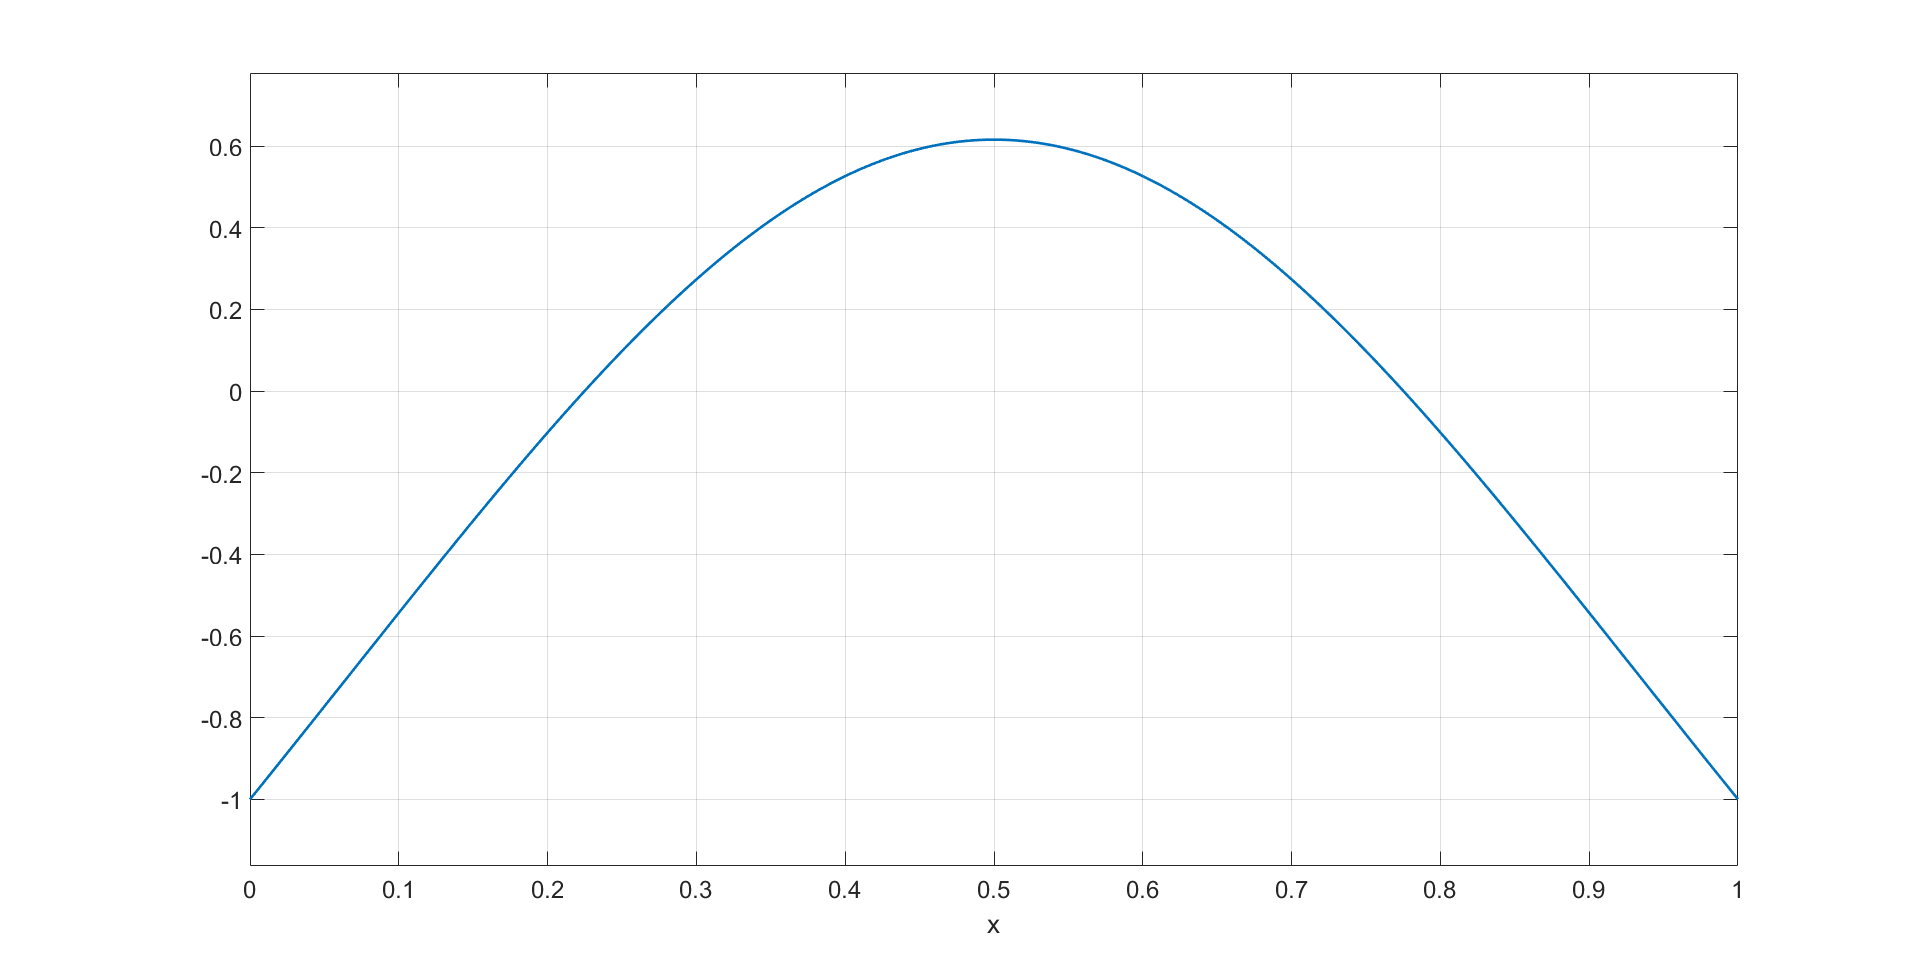
\includegraphics[width=1\linewidth]{Free1.png}
			\subcaption{ $\lambda_1 = 1.544$, $B_1 = -1.022$}
			\label{fig:minipage2}
		\end{minipage}
		\begin{minipage}[b]{0.7\linewidth}
			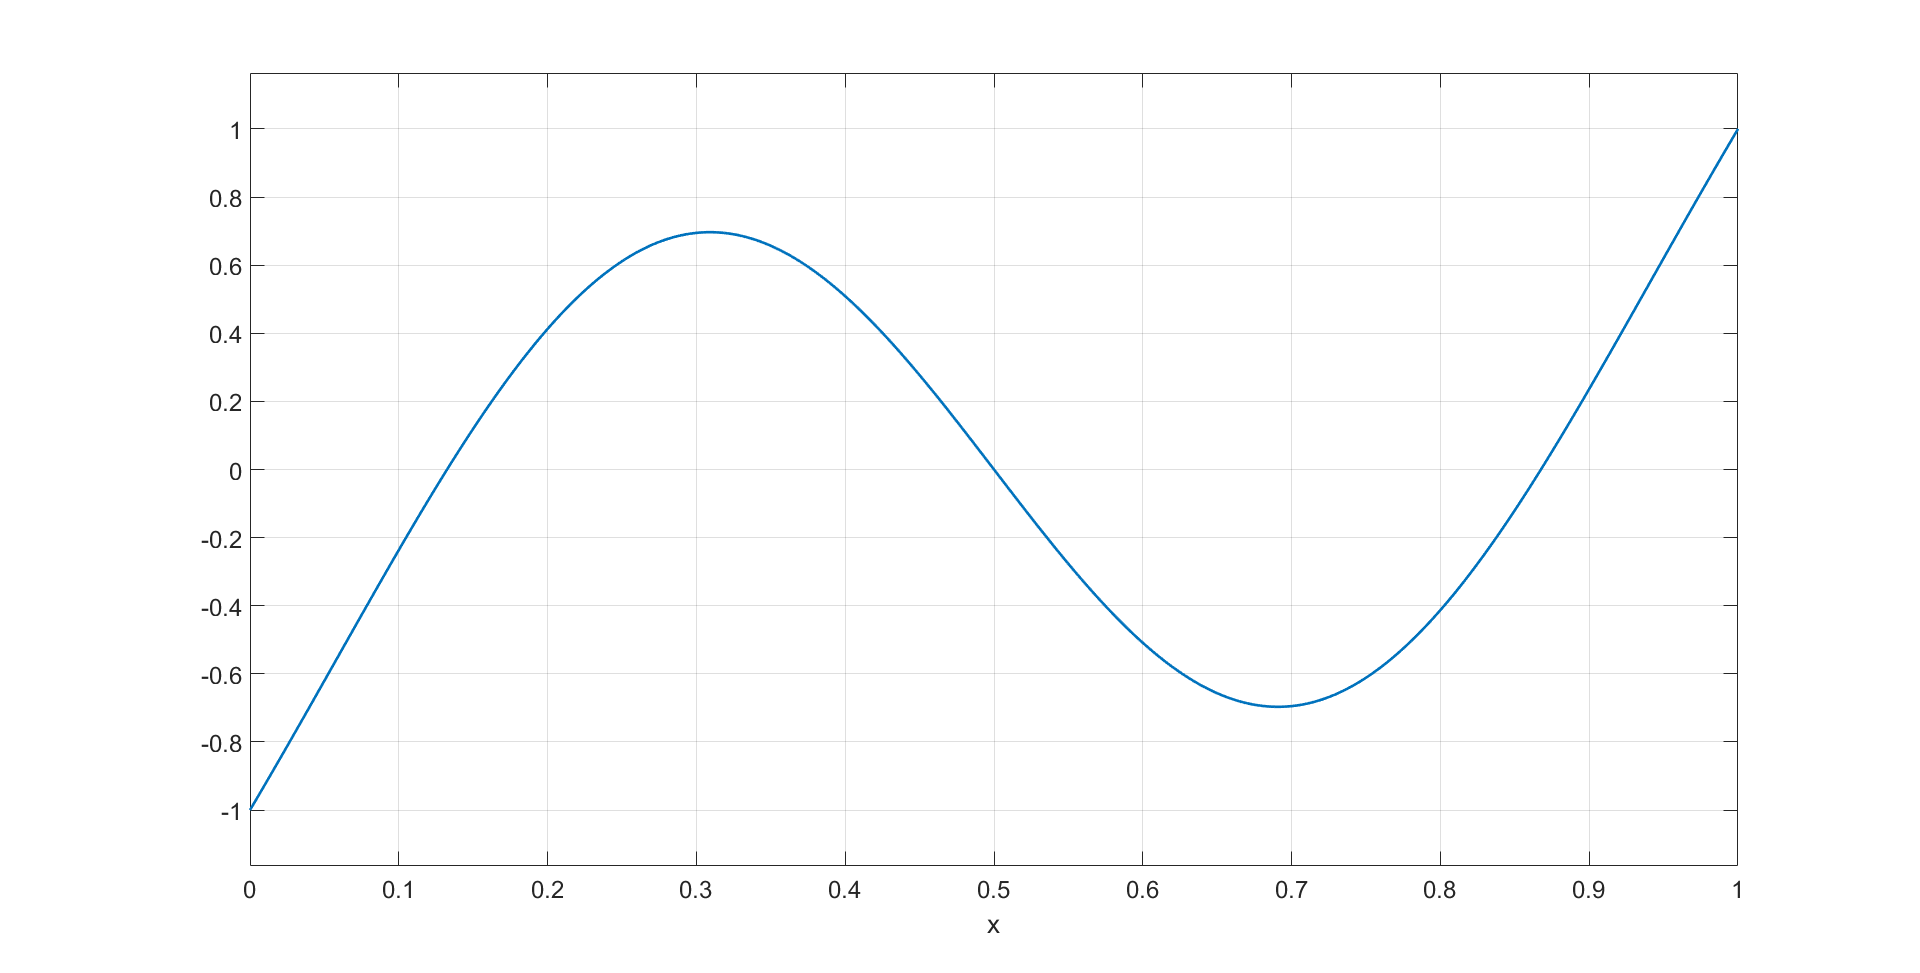
\includegraphics[width=1\linewidth]{Free2.png}
			\subcaption{$\lambda_2 = 10.26$, $B_2 = -0.9982$}
			\label{fig:minipage1}
		\end{minipage}
	}
	
	\makebox[\textwidth][c]{
		\centering
		\begin{minipage}{.7\textwidth}
			\centering
			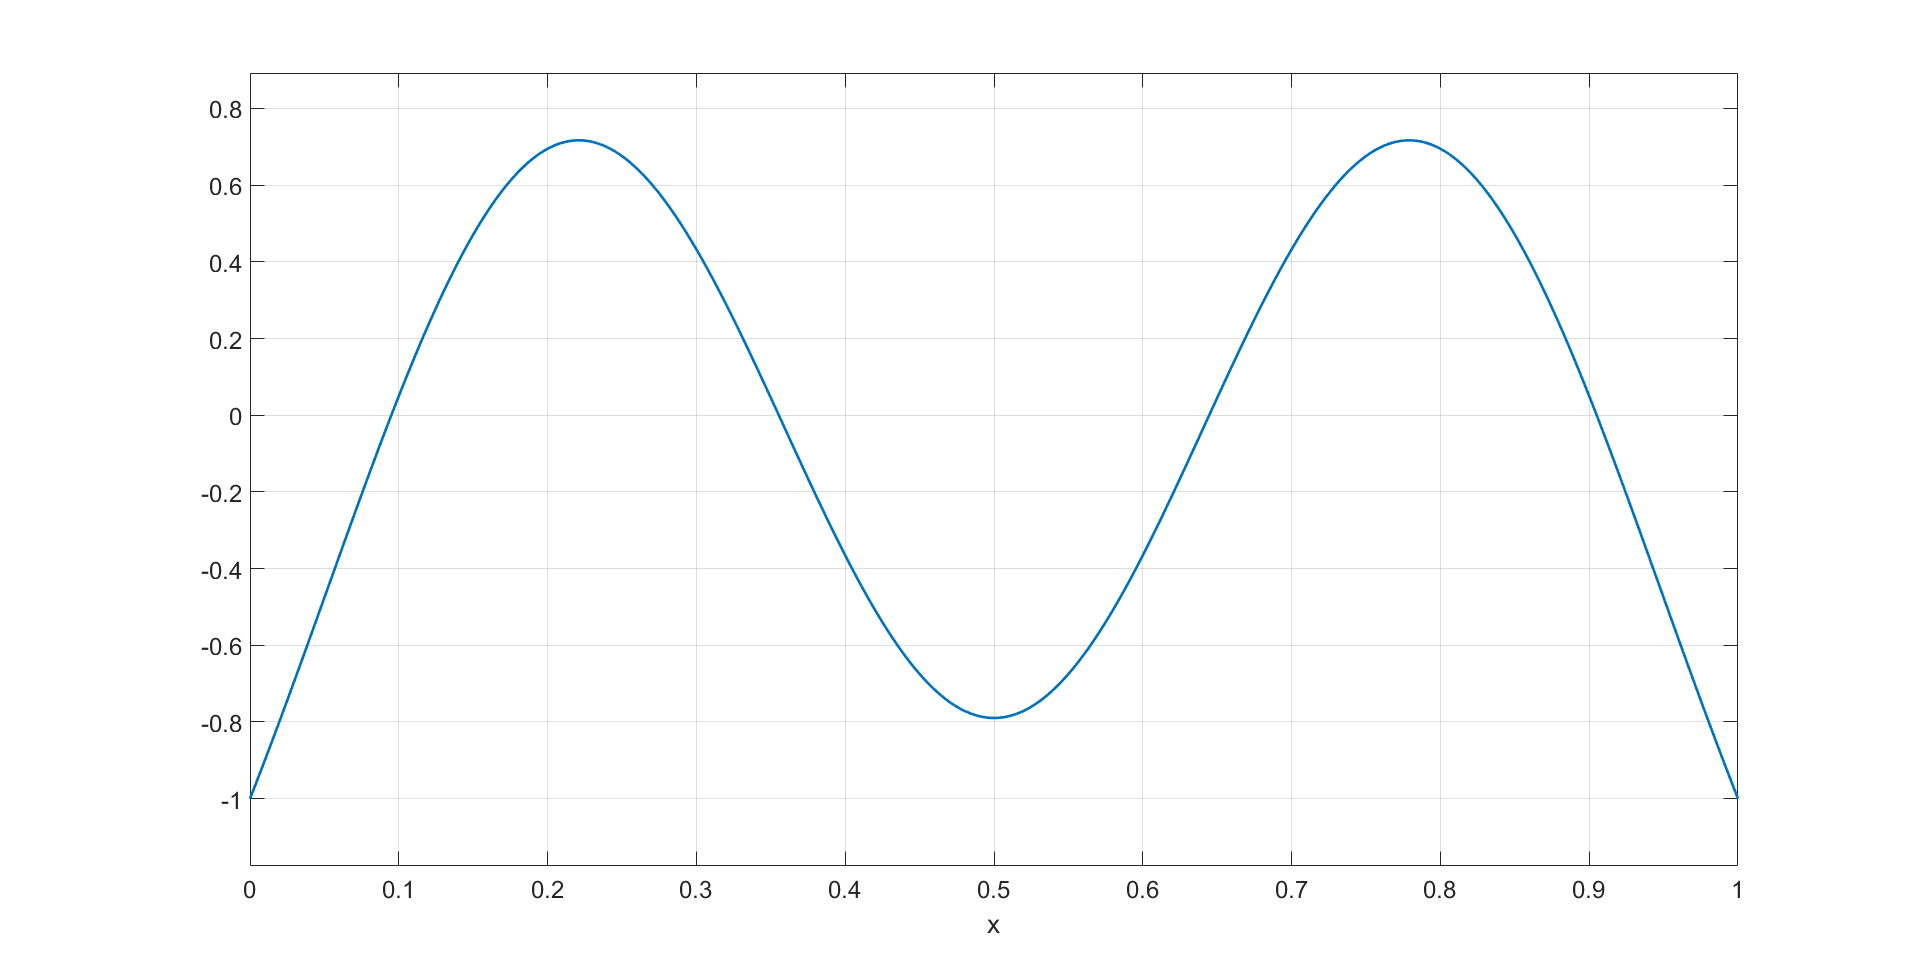
\includegraphics[width=1\linewidth]{Free3.png}
			\subcaption{$\lambda_3 = 33.41$, $B_3 = -1.000$}
			\label{fig:minipage1}
		\end{minipage}
		\begin{minipage}{.7\textwidth}
			\centering
			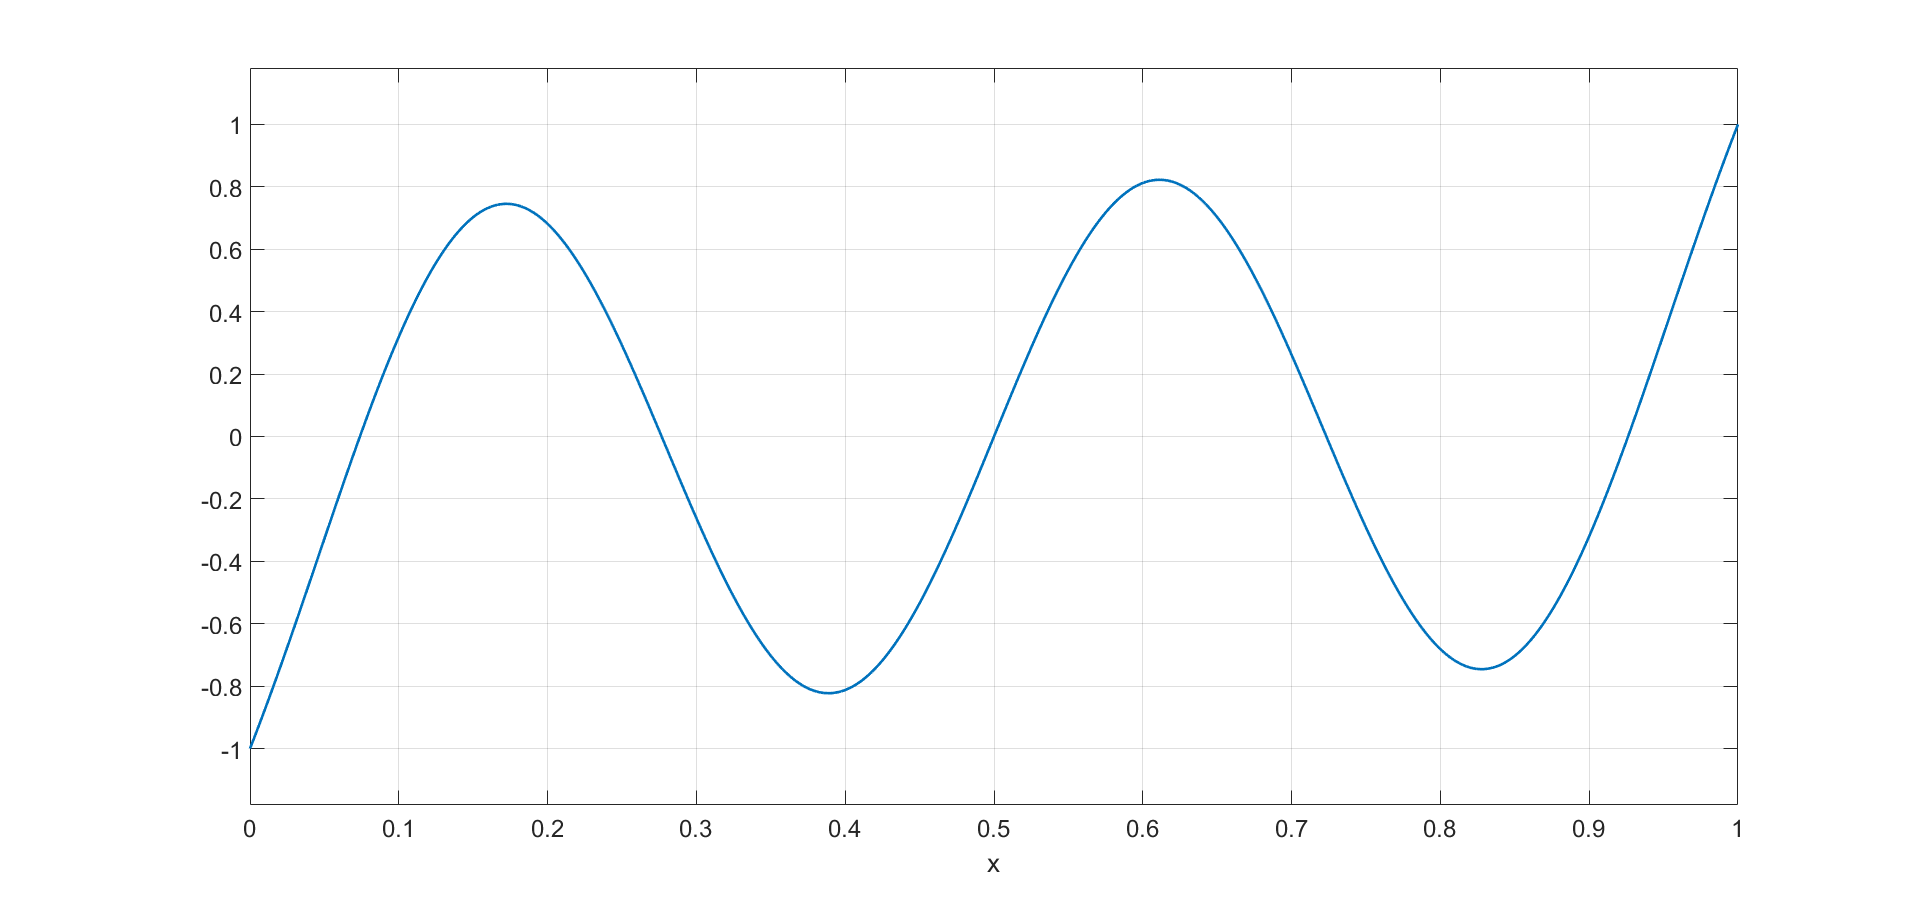
\includegraphics[width=1\linewidth]{Free4.png}
			\subcaption{$\lambda_4 = 76.16$, $B_4 = -0.9999$}
			\label{fig:minipage2}
		\end{minipage}
	}
	\caption{Sketch of $w$ of the first 4 mode shapes of the free-free beam. $\alpha = 1200$ and $\gamma = 0.25$ with $A_k = 1$.}
\end{figure}
\FloatBarrier
\begin{figure}[h!]
	
	\makebox[\textwidth][c]{
		\centering
		\begin{minipage}[b]{0.7\linewidth}
			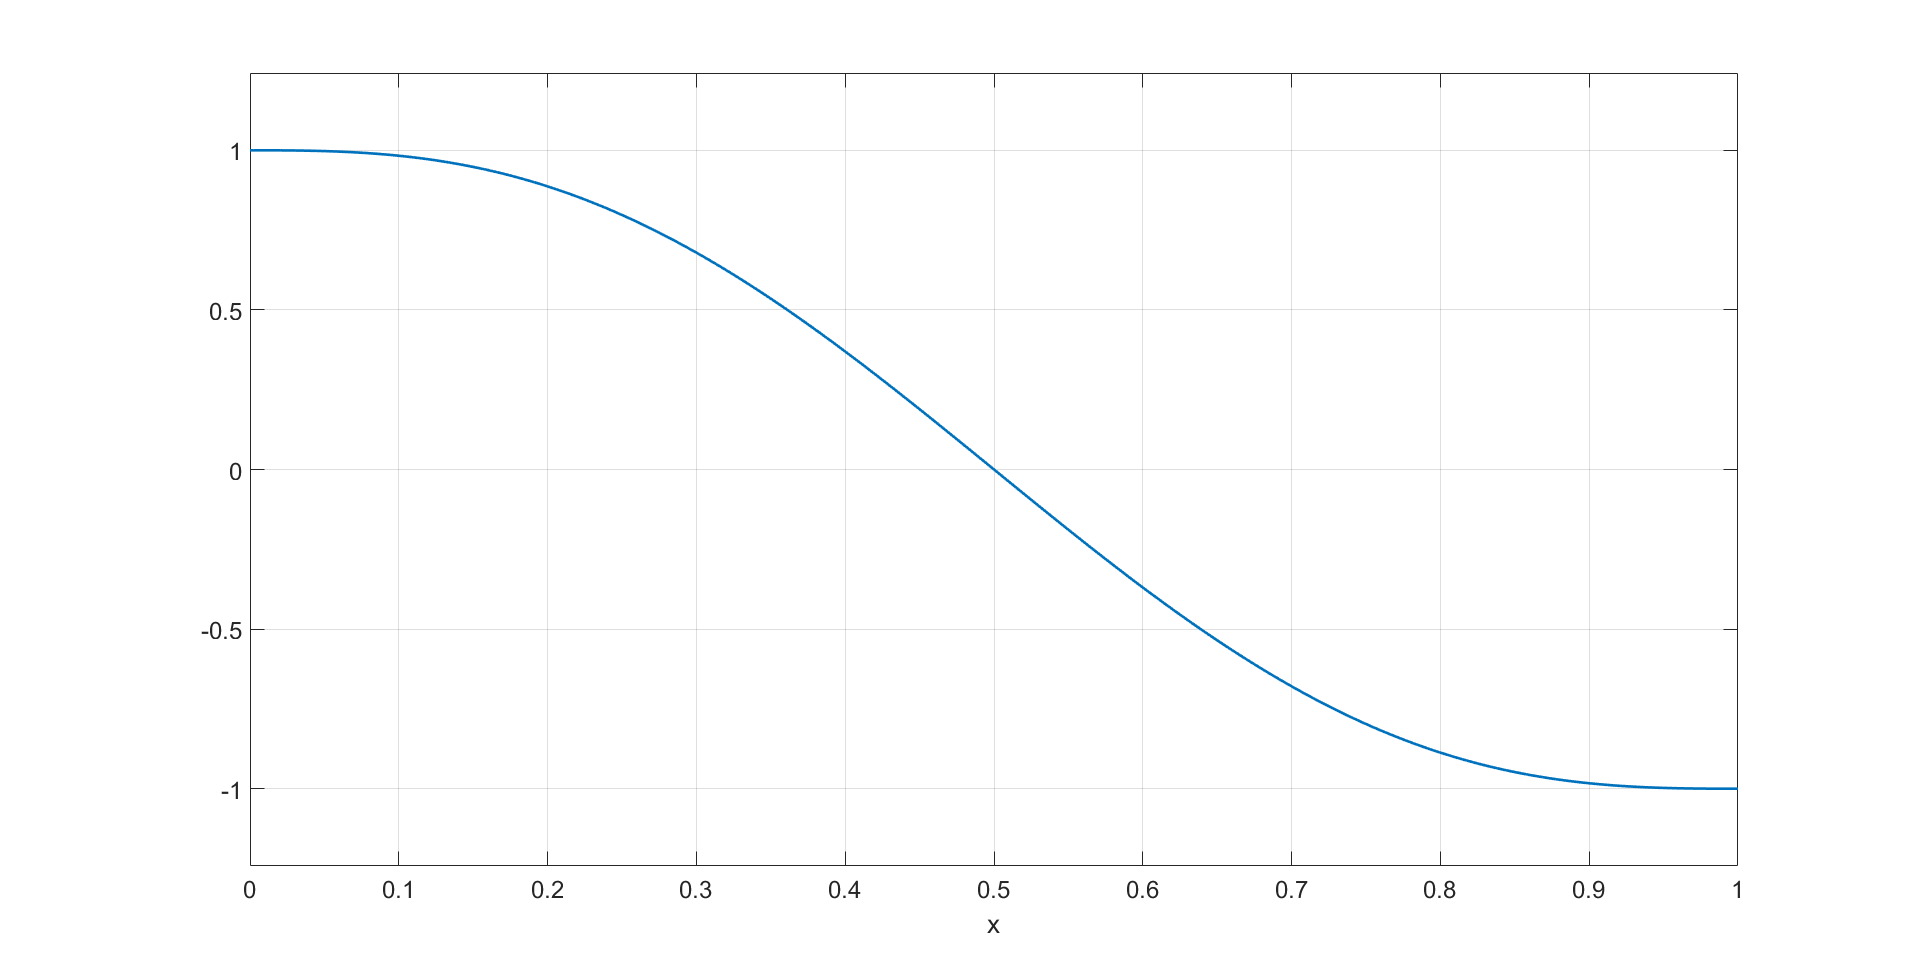
\includegraphics[width=1\linewidth]{Free21.png}
			\subcaption{ $\lambda_2 = 1.544$, $B_1 = -1.022$}
			\label{fig:minipage2}
		\end{minipage}
		\begin{minipage}[b]{0.7\linewidth}
			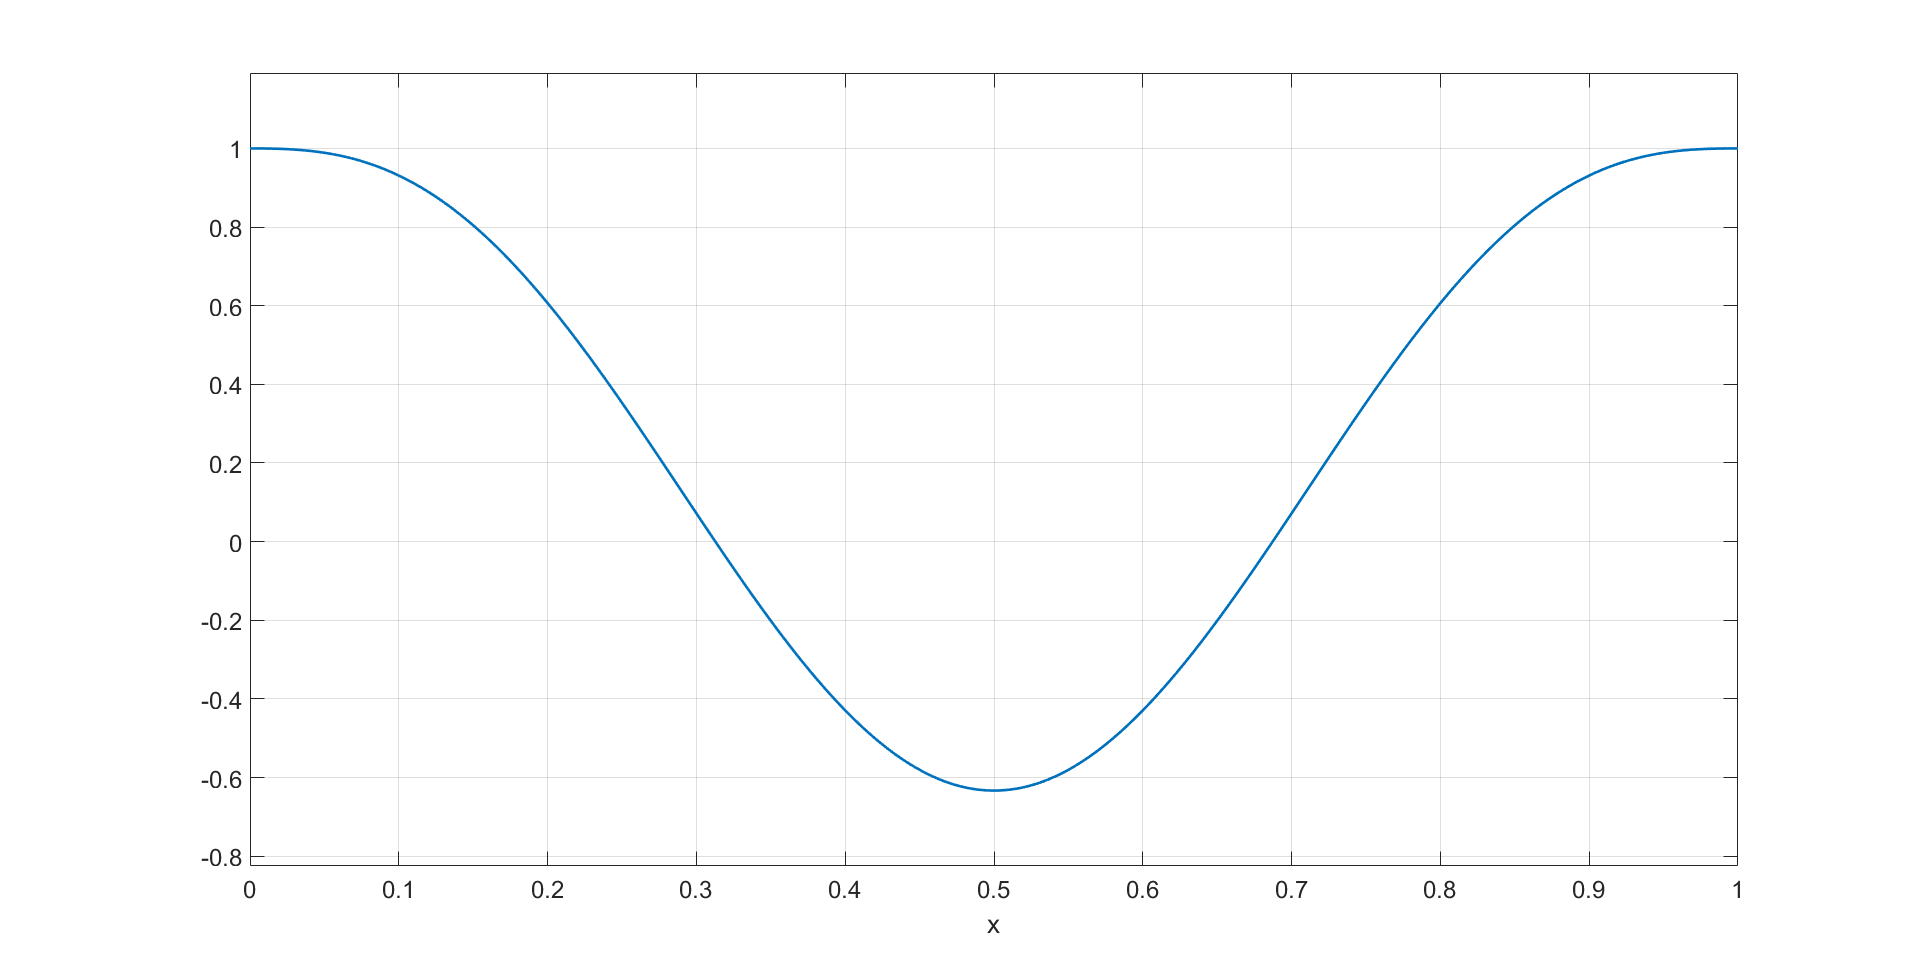
\includegraphics[width=1\linewidth]{Free31.png}
			\subcaption{$\lambda_3 = 10.26$, $B_2 = -0.9982$}
			\label{fig:minipage1}
		\end{minipage}
	}
	
	\caption{Sketch of $\phi$ for the first two mode shapes of the free-free beam. $\alpha = 1200$ and $\gamma = 0.25$ with $A_k = 1$.}
\end{figure}
\FloatBarrier

The motivation for the free-free beam in this dissertation is section 4.6. In this section, an article is discussed in which the eigenvalues of a free-free Timoshenko beam are compared to empirical results from an experiment conducted in [SP06].

\end{document}
